

%Version 3.1 December 2024
% See section 11 of the User Manual for version history
%
%%%%%%%%%%%%%%%%%%%%%%%%%%%%%%%%%%%%%%%%%%%%%%%%%%%%%%%%%%%%%%%%%%%%%%
%%                                                                 %%
%% Please do not use \input{...} to include other tex files.       %%
%% Submit your LaTeX manuscript as one .tex document.              %%
%%                                                                 %%
%% All additional figures and files should be attached             %%
%% separately and not embedded in the \TeX\ document itself.       %%
%%                                                                 %%
%%%%%%%%%%%%%%%%%%%%%%%%%%%%%%%%%%%%%%%%%%%%%%%%%%%%%%%%%%%%%%%%%%%%%

%%\documentclass[referee,sn-basic]{sn-jnl}% referee option is meant for double line spacing

%%=======================================================%%
%% to print line numbers in the margin use lineno option %%
%%=======================================================%%

%%\documentclass[lineno,pdflatex,sn-basic]{sn-jnl}% Basic Springer Nature Reference Style/Chemistry Reference Style

%%=========================================================================================%%
%% the documentclass is set to pdflatex as default. You can delete it if not appropriate.  %%
%%=========================================================================================%%

%%\documentclass[sn-basic]{sn-jnl}% Basic Springer Nature Reference Style/Chemistry Reference Style

%%Note: the following reference styles support Namedate and Numbered referencing. By default the style follows the most common style. To switch between the options you can add or remove �Numbered� in the optional parenthesis. 
%%The option is available for: sn-basic.bst, sn-chicago.bst%  
 
%%\documentclass[pdflatex,sn-nature]{sn-jnl}% Style for submissions to Nature Portfolio journals
%%\documentclass[pdflatex,sn-basic]{sn-jnl}% Basic Springer Nature Reference Style/Chemistry Reference Style
\documentclass[pdflatex,sn-mathphys-num]{sn-jnl}% Math and Physical Sciences Numbered Reference Style
%%\documentclass[pdflatex,sn-mathphys-ay]{sn-jnl}% Math and Physical Sciences Author Year Reference Style
%%\documentclass[pdflatex,sn-aps]{sn-jnl}% American Physical Society (APS) Reference Style
%%\documentclass[pdflatex,sn-vancouver-num]{sn-jnl}% Vancouver Numbered Reference Style
%%\documentclass[pdflatex,sn-vancouver-ay]{sn-jnl}% Vancouver Author Year Reference Style
%%\documentclass[pdflatex,sn-apa]{sn-jnl}% APA Reference Style
%%\documentclass[pdflatex,sn-chicago]{sn-jnl}% Chicago-based Humanities Reference Style

%%%% Standard Packages
%%<additional latex packages if required can be included here>

\usepackage{graphicx}%
\usepackage{multirow}%
\usepackage{amsmath,amssymb,amsfonts}%
\usepackage{amsthm}%
\usepackage{mathrsfs}%
\usepackage[title]{appendix}%
\usepackage{xcolor}%
\usepackage{textcomp}%
\usepackage{manyfoot}%
\usepackage{booktabs}%
\usepackage{algorithm}%
\usepackage{algorithmicx}%
\usepackage{algpseudocode}%
\usepackage{listings}%
%%%%

%%%%%=============================================================================%%%%
%%%%  Remarks: This template is provided to aid authors with the preparation
%%%%  of original research articles intended for submission to journals published 
%%%%  by Springer Nature. The guidance has been prepared in partnership with 
%%%%  production teams to conform to Springer Nature technical requirements. 
%%%%  Editorial and presentation requirements differ among journal portfolios and 
%%%%  research disciplines. You may find sections in this template are irrelevant 
%%%%  to your work and are empowered to omit any such section if allowed by the 
%%%%  journal you intend to submit to. The submission guidelines and policies 
%%%%  of the journal take precedence. A detailed User Manual is available in the 
%%%%  template package for technical guidance.
%%%%%=============================================================================%%%%

%% as per the requirement new theorem styles can be included as shown below
\theoremstyle{thmstyleone}%
\newtheorem{theorem}{Theorem}%  meant for continuous numbers
%%\newtheorem{theorem}{Theorem}[section]% meant for sectionwise numbers
%% optional argument [theorem] produces theorem numbering sequence instead of independent numbers for Proposition
\newtheorem{proposition}[theorem]{Proposition}% 
%%\newtheorem{proposition}{Proposition}% to get separate numbers for theorem and proposition etc.

\theoremstyle{thmstyletwo}%
\newtheorem{example}{Example}%
\newtheorem{remark}{Remark}%

\theoremstyle{thmstylethree}%
\newtheorem{definition}{Definition}%

\raggedbottom
%%\unnumbered% uncomment this for unnumbered level heads

\begin{document}

\title[Climate Change Pulse: An Agentic RAG-Enhanced Framework for Interactive Sentiment Analysis and Global Disaster Data Visualization]{Climate Change Pulse: An Agentic RAG-Enhanced Framework for Interactive Sentiment Analysis and Global Disaster Data Visualization}

%%=============================================================%%
%% GivenName	-> \fnm{Joergen W.}
%% Particle	-> \spfx{van der} -> surname prefix
%% FamilyName	-> \sur{Ploeg}
%% Suffix	-> \sfx{IV}
%% \author*[1,2]{\fnm{Joergen W.} \spfx{van der} \sur{Ploeg} 
%%  \sfx{IV}}\email{iauthor@gmail.com}
%%=============================================================%%

\author*[1]{\fnm{Alan} \sur{Zheng}}\email{alanzheng240@gmail.com}

\author[ ]{\fnm{Carlos} \sur{Gonzalez}}\email{carlos01oscar@gmail.com}
%\equalcont{These authors contributed equally to this work.}

%\author[1,2]{\fnm{Third} \sur{Author}}\email{iiiauthor@gmail.com}
%\equalcont{These authors contributed equally to this work.}

\affil*[1]{\orgdiv{West-Windsor Plainsboro High School North}, \orgaddress{\street{90 Grovers Mill Rd}, \city{Plainsboro Township}, \postcode{08536}, \state{NJ}, \country{USA}}}

\affil[2]{\orgdiv{Computer Science Department}, \orgname{California State Polytechnic University}, \orgaddress{\postcode{91768}, \state{CA}, \country{USA}}}

%\affil[3]{\orgdiv{Department}, \orgname{Organization}, \orgaddress{\street{Street}, \city{City}, \postcode{610101}, \state{State}, \country{Country}}}

%%==================================%%
%% Sample for unstructured abstract %%
%%==================================%%

\abstract{
    Climate change is an urgent global issue, with natural disasters becoming more severe and frequent due to human activities. Understanding public sentiment around these events can inform climate awareness and policy. We developed Climate Change Pulse, a web-based tool that visualizes natural disasters alongside Twitter data to analyze how proximity and time influence climate-related sentiments. Using the Climate Change Twitter Dataset, we examined over 15 million tweets, mapping them with disaster data through an interactive UI.
Challenges included missing geospatial data and sentiment classification limitations, addressed by refining data filters and leveraging embedded tweets. Our experiments tested how distance and time around disasters affect sentiment, revealing that proximity intensifies negative emotions, and climate change deniers exhibit surprisingly strong negative sentiments. Compared to prior methodologies focused on data collection or basic sentiment analysis, our approach emphasizes user interactivity and behavioral analysis. Climate Change Pulse offers a dynamic way to understand climate discourse, bridging data insights with public engagement.
}

%%================================%%
%% Sample for structured abstract %%
%%================================%%

% \abstract{\textbf{Purpose:} The abstract serves both as a general introduction to the topic and as a brief, non-technical summary of the main results and their implications. The abstract must not include subheadings (unless expressly permitted in the journal's Instructions to Authors), equations or citations. As a guide the abstract should not exceed 200 words. Most journals do not set a hard limit however authors are advised to check the author instructions for the journal they are submitting to.
% 
% \textbf{Methods:} The abstract serves both as a general introduction to the topic and as a brief, non-technical summary of the main results and their implications. The abstract must not include subheadings (unless expressly permitted in the journal's Instructions to Authors), equations or citations. As a guide the abstract should not exceed 200 words. Most journals do not set a hard limit however authors are advised to check the author instructions for the journal they are submitting to.
% 
% \textbf{Results:} The abstract serves both as a general introduction to the topic and as a brief, non-technical summary of the main results and their implications. The abstract must not include subheadings (unless expressly permitted in the journal's Instructions to Authors), equations or citations. As a guide the abstract should not exceed 200 words. Most journals do not set a hard limit however authors are advised to check the author instructions for the journal they are submitting to.
% 
% \textbf{Conclusion:} The abstract serves both as a general introduction to the topic and as a brief, non-technical summary of the main results and their implications. The abstract must not include subheadings (unless expressly permitted in the journal's Instructions to Authors), equations or citations. As a guide the abstract should not exceed 200 words. Most journals do not set a hard limit however authors are advised to check the author instructions for the journal they are submitting to.}

\keywords{Natural Language Processing, Machine Learning, Sentiment, Disasters}

%%\pacs[JEL Classification]{D8, H51}

%%\pacs[MSC Classification]{35A01, 65L10, 65L12, 65L20, 65L70}

\maketitle

\section{Results}
In the experiment, we aimed to test how distance and time windows around natural disasters influence public sentiment on climate change as expressed on Twitter. We systematically varied distance thresholds (500 km, 1000 km, 2000 km) and time windows (1, 3, and 7 days before and after a disaster) to identify patterns. Using the Climate Change Twitter Dataset, we filtered tweets based on proximity and time relative to disasters and calculated average sentiment scores.

Our most significant findings showed that tweets closer to disasters tend to have stronger negative sentiments, highlighting the emotional impact of proximity. Sentiment also became more negative as time progressed after a disaster, reflecting prolonged concern. Interestingly, climate change deniers exhibited the most negative sentiment, even more than believers, which was unexpected. This suggests emotional responses are influenced by both proximity to disasters and pre-existing beliefs. The experiment underscored the importance of parameter selection and revealed complex interactions between distance, time, and user stance.

\section{Preview}
The approach outlined by Barachi, May El, et. al used a Bi-directional LSTM model for sentiment classification on climate-related social media data. It effectively categorized sentiments but relied heavily on API data collection, which we lacked. Its focus was limited to model training, while our project advanced this by analyzing already labeled data for deeper insights.

The proposed method for Lu, Yafeng, et. al. visualized social media sentiment during disasters, using geographic data from the Ebola Twitter dataset. While effective in mapping sentiment, it lacked user interactivity and broader analytical factors. Our project improved on this with a user-friendly UI and an emphasis on behavioral differences between climate change deniers and believers.

Mouronte-López and Subirán analyzed climate change sentiments on Twitter using sentiment models like VADER and topic modeling. Although comprehensive, it didn’t explore user behavior or disaster proximity effects. Climate Change Pulse builds on this by integrating interactive visualizations and focusing on how disasters influence sentiment over time and space.

Drawing lessons from existing methods, our project moved beyond the limitations of traditional RAG and fixed data collection by adopting an agentic RAG framework for dynamically generating SQL queries on our static, tabular disaster and tweet data. This strategic shift makes use of the iterative nature and multi-domain capabilities of agentic systems, enabling a more interactive and behavior-focused conversational chatbot than approaches centered on basic sentiment classification or static visualizations.


\section{Introduction}\label{sec1}
\subsection{Introduction to Problem}\label{subsec2}
Climate change is one of the most prominent, terrible issues we are facing right now. Extreme heat and climate change induced natural disasters directly and indirectly impact people worldwide.
Climate change from human activities causes disasters to be more intense and frequent. Hot seasons now keep breaking record temperature and worse heat waves, floods and droughts are normal in many countries. Ice sheets are melting, ocean levels are rising and warmer oceans create bigger hurricanes. Importantly, with the rising temperature, tipping points, changes in systems are passed which are irreversible. From The Climate Book by Greta Thunberg “IPCC estimates that global warming will reach 3.2°C by 2100”. When Hurricane Sandy hit New York, 8 billion dollars of damage from the storm surge were because of climate change. In 2003, a heatwave in Europe caused more than 70000 premature deaths, and climate change has doubled the chance of occurrence. If global warming is under 2°C over 50 years, it could prevent 4.5 million premature deaths in the U.S alone.
Technology can give us information about peoples ideas–tools like data analysis can assess people’s perception of different issues. For climate change, how would being near a disaster impact a person's emotions, or their sentiment? And how can we use data from social media platforms such as X, formerly known as Twitter?  Answering these questions is key to better inform the general public to help drive change in policy-making in our society. 
Present examples in tweets show potential areas of interest that we aim to further explore. We aim to observe whether natural disasters amplified by climate change impact people's sentiment. Compared to surveys that evaluate people's stance and awareness on current issues, people tend to express themselves more intensely and personally. This advantage is because social media is a less formal environment. Additionally, social media has more younger users and can be more diverse than sample populations used in surveys. As seen from the Pew Research Center report in 2023, when observing user activity among various social platforms such as TikTok, Instagram, Snapchat, YouTube, and Facebook, “a third of teens use at least one of these five sites almost constantly.” This advantageous presentation of information is what allows us to extract more meaningful insights from the readily collected data.

\subsection{Method Proposal}\label{subsec3}

Climate Change Pulse is a web tool that visualizes disasters onto a world map, overlaid by various different tweets. There is a scroll feature for the user to visualize which natural disasters occurred per year. Red dots on the map indicate a recorded disaster, and upon selection, tweets within a 1000 mile radius to the disaster will be displayed. The world map combines tools such as javascript and d3 from the following github repository.
Our research aims to use the datasets to see if there are any connections between sentiment and disaster. Both the tweets and disaster data were pooled from the “Climate Change Twitter Dataset” research initiative by Dimitrios Effrosynidis et al. (2022). Over fifteen million data points spanning over thirteen years related to climate change were sourced from the social media platform, where data such as gender, stance, sentiment, and disaster type are included. The tweets are from different people and organizations but are all talking about climate change. 


\section{Challenges}\label{sec2}
In order to build the project, a few challenges have been identified as follows.
\subsection{World Map Interface Integration}\label{subsec4}
One primary challenge is incorporating the dataset with the world map interface. For example, the world map has a dropdown menu showing the name of all the countries, however some countries have different naming in the datasets. This would have to be dealt with because it can cause issues in the pairing of those countries and the tweets in the area. Other data is also formatted so javascript code cannot work with it. The disaster data’s date records needed to be converted into standardized date-formated to work with the code. Additionally creating the interface itself has its own challenges. Disasters are represented with some icons, and the map needs to be constantly updated to remove old icons and add new icons. Also, ever since Elon Musk acquired twitter, the data can’t be accessed directly. This means getting the contents of tweets by hydrating them is no longer viable.
\subsection{Twitter Data Accessibility}\label{subsec5}
Another challenge was ensuring twitter and disaster data was properly structured and accessible for analysis. A significant portion of data had incomplete properties, so they can’t be visualized. Missing latitude and longitude values means that tweets and disasters can’t be placed on the map. This means that in order to render the data, we would have to preprocess it by parsing dates, grouping records and filtering invalid entries. At the same time, if we filtered out invalid entries it excludes a substantial portion of the data which is misleading. So an approach to get usable data would also need methods to fill in errors in order to keep as much data as possible.
\subsection{RAG Architecture}\label{subsec6}
When deciding on the architecture of our LLM, we explored different methods, such as large-context windows and fine-tuned LLMs. We’ve opted for a RAG-based solution, instructing the model to act as a “data analyst” to interact with the dataset. Due to the complexity of the task, and the limitations of accessible data, training and fine-tuning a model seemed less promising compared to the RAG-based solution, where all we need to do is instruct the LLM to generate queries to index our data. We also considered the advantages and drawbacks between an in-memory pandas dataframe versus an out-of-memory SQLite database. Due to the limitations of available cloud-computing resources, and the performance differences for this specific task, designing an LLM to generate SQL queries made more sense for the task of retrieving data efficiently and accurately.

\section{System Overview}\label{sec3}
The web application is a map visualization tool with a conversational chatbot. can change the year and observe differences in tweet sentiment and disaster severity  across various countries. When the user clicks on a disaster, the system will collect from the tweets dataset and select those within a specific time and distance.  For more clarification, the user can ask context-driven questions regarding the dataset.
The data was grouped based on attributes as year and country, a map object was created to efficiently store tweets based on ID. The visualization update function incorporates the data to be displayed. We fill in missing data points from our dataset using the Google Maps API. Notably, we fill in the missing latitude and longitudinal coordinates by using the region / address a disaster has occurred–that way, we ensure that we can overlay every disaster into the visualization. We used a Google Maps API key to find the locations based on the data and calculated the coordinates. We also worked more on the data, we removed tweets from the twitter data that didn’t have coordinates. Due to the large sample size, and the lack of other geospatial information from the Twitter dataset, finding the location for these tweets was not possible.
Pandas was used for extensive data visualization and analysis  to better understand the underlying distributions and patterns in the data. For example, one visualization  compared the mean sentiment of tweets and their aggressiveness with the worst disasters. The purpose of showing tweets when you click on a disaster is to see if there are changes in sentiment. Specifically, to see if being near a disaster around the time of it is related to sentiment on climate change.

\begin{figure}[h]
\centering
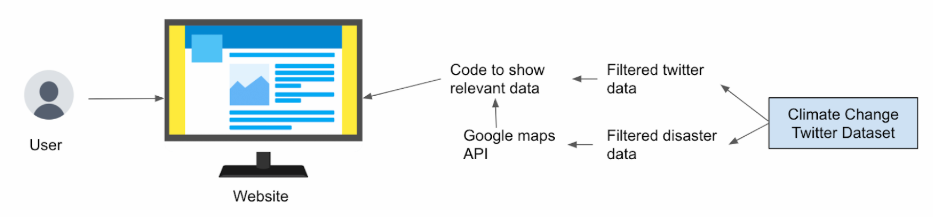
\includegraphics[width=12cm]{images/climatechangepulse.PNG}
\caption{Flowchart showing the code for the application}
\end{figure}

\subsection{Component A}\label{subsec7}
On the website cooler countries are in shades blue while hotter countries are in shades of red. The symbols used for the disaster are red dots, when the map is running they “flicker” on and off. Hovering over a disaster also gives information of the number of deaths from the disaster. In order to show the tweets for disasters windows are used, the windows have a scroll feature to see all the embedded tweets. To get out of a tweet window click out of the window or on another disaster.


The embedTweets function expects a numpy array of tweet id’s as its parameter. This function is immediately called upon execution of the program, when the website is first launched. It uses the tweetsElement array which is in code dealing with the twitter data. After that it has some attributes that affect the appearance of the embedded tweets. Setting conversation to none means it doesn’t show replies to the tweet. Cards hide images and polls that the tweet would have. Align centers the tweet and theme makes the tweet in light mode.

\begin{figure}[h]
\centering
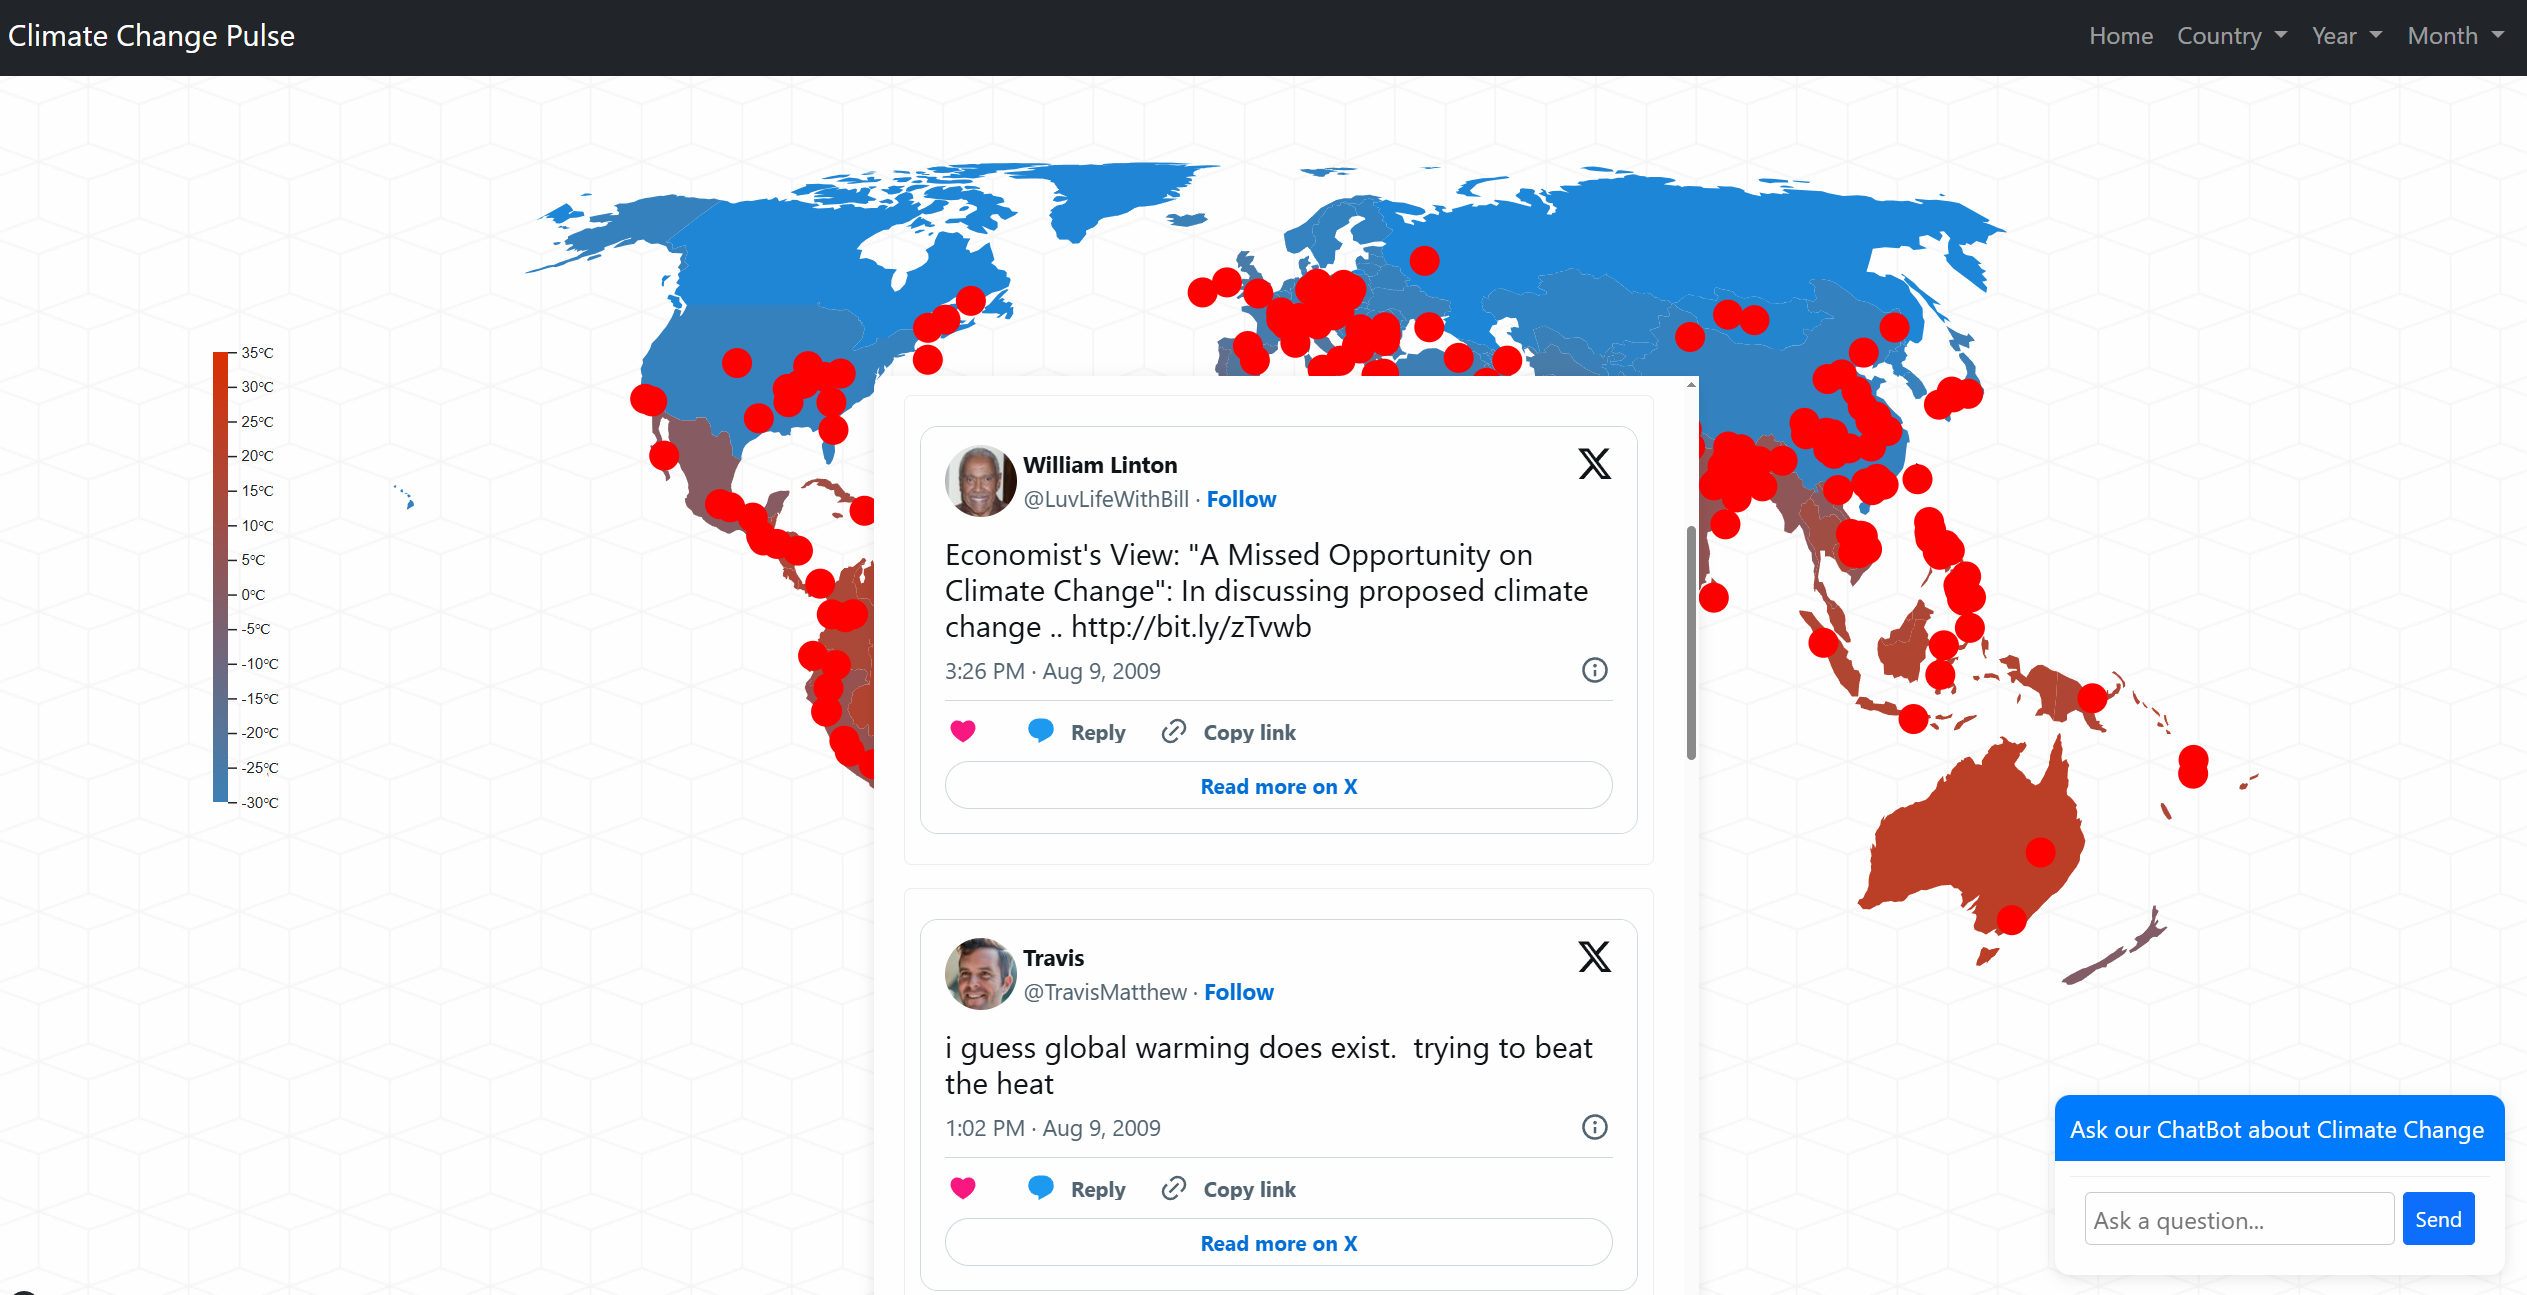
\includegraphics[width=12cm]{images/climatechangepulse3.PNG}
\caption{Climate Change Pulse web application interface}
\end{figure}

\subsection{Component B}\label{subsec8}
Many data points in the disaster data were missing coordinates which meant the data wasn’t a complete recommendation. However many disasters have a geographic location. Using google maps API we checked the location of the data to find possible locations. Then taking all of those location’s coordinates into account we got the average.

\begin{figure}
\centering
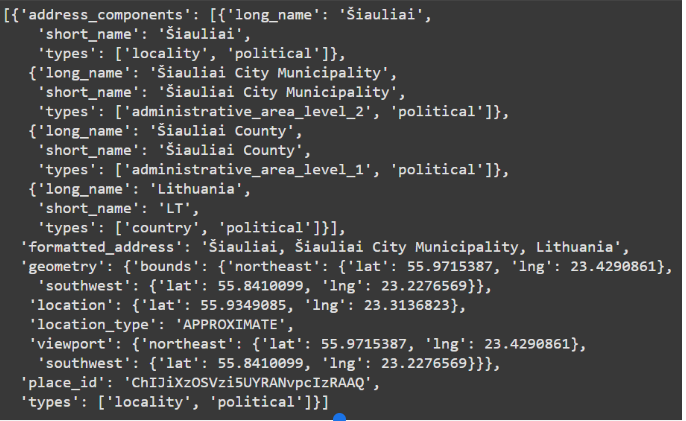
\includegraphics[width=7cm]{images/climatechangepulse4.PNG}
\caption{Example of possible locations after calling geocode function}
\end{figure}

In get\_coords we are calling the google maps geocode function to get possible locations, then adding it to latitude and longitude sets. Afterwards we get the average latitude and longitudes. Also some locations have special characters so we had to encode and decode it using two character encoding standards. Finally the modified data is added back into the data file.


\subsection{Component C}\label{subsec9}
We were particularly interested in answering the following question: When a disaster occurs, does this increase the discussion of climate change in the region? Combining the tools of programming with the large corpus of data, we aim to further explore the data itself by performing various exploratory data analysis techniques, such as aggregating, filtering, augmenting the data to paint a clearer picture of the granularity of the datasets.

We utilize the matplotlib module in python to create this comprehensive visualization, which is an example of several graphs we generated to better understand the underlying contents of the data. Several tasks needed to be completed, such as aggregating the sentiment and aggressiveness scores into months per year; labeling the extreme points in the disasters dataset, such as the most costly disaster (the amount, in USD, incurred in damages as a result to the disaster); most deaths occurred; and most people affected. We then overlaid a line plot of the mean sentiment and aggressiveness scores onto a graph, where the shaded in regions indicate our disaster points of interest. Once all these data points are collected, we simply combine all the data into this one graph.

\begin{figure}[H]
\centering
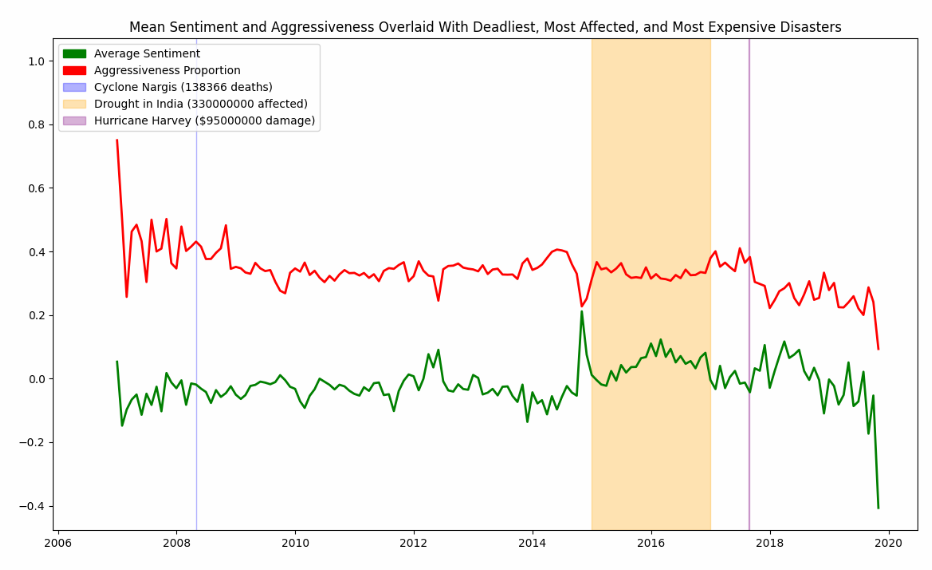
\includegraphics[width=12cm]{images/climatechangepulse5.PNG}
\caption{Line plot of twitter sentiment and aggressiveness data and disasters of interest}
\end{figure}

\newpage

\subsection{Component D}\label{subsec10}
The AI feature is a contextually-aware RAG-based system, where the user can ask questions about the datasets and receive accurate up-to-date information about the data. We firstly load the databases in-memory using sqlite, retrieving the column names and rows from the original sources files, and loading them into two separate databases.The program checks the database to determine which one is appropriate to use, given some user query, to then generate a SQL query. Next, the system validates the SQL expression, retrying if it's invalid or can’t be parsed. We provide error handling for instances such as these, ensuring the LLM can revise its mistakes upon future iteration. The LLM is presented with metadata from the databases , such as the column names, data types, and granularity to ensure accurate retrieval of information. We ultimately are looking at the use-case of LLM’s to query and interact with large databases, exploring the possibilities of LLMs assisting distributed systems to answer users' questions via an agentic framework.

\begin{figure}[H]
\centering
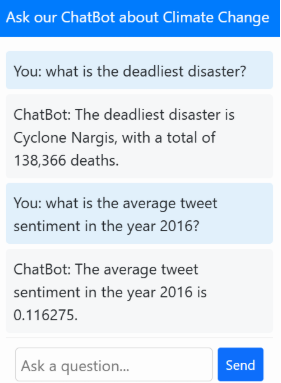
\includegraphics[width=4cm]{images/climatechangepulse6.PNG}
\caption{Example of a conversation with AI feature}
\end{figure}

We ask the LLM to generate a SQL query based on the user’s query and dataset of choice. We call the answer\_with\_table function which takes in the user query and returns a SQL expression that retrieves the information required to answer the user query. The LLM could fail to retrieve information because of errors, due to a nonsensical query received from the user (e.g.: ‘Please tell me about my finances.’), or a fault from the LLM (e.g.: we index from a column which doesn’t exist in the database.). We consider these scenarios by feeding the LLM error feedback, and modify the prompt to attempt to generate a new query. The retry\_count variable keeps track of the amount of attempts so they don’t exceed max\_retries. This process continues until we either successfully retrieve information from the database, or until we fallback to some error. The LLM prompts the user with updated information about their query, with the client receiving a textual response.
\newpage

\section{Experiment}\label{sec4}
A potential blind spot in the program is the selection of distance and time windows around disasters. If the chosen thresholds (e.g., 500 km, 1000 km, or 2000 km) are too narrow or too broad, they might miss key sentiment patterns or dilute meaningful insights. It’s critical to test these parameters to ensure the program accurately captures the relationship between disasters and public sentiment.

To test the impact of distance and time windows, the experiment systematically varies these parameters. Distance thresholds are set at 500 km, 1000 km, and 2000 km, while time windows are defined as 1, 3, and 7 days before and after a disaster. These ranges are chosen to reflect realistic geographical and temporal scopes of disaster impact.

The experiment uses the "Climate Change Twitter Dataset" by Dimitrios Effrosynidis et al. (2022), which includes over 15 million tweets related to climate change. Control data is sourced from the same dataset, ensuring consistency in tweet sentiment, stance, and disaster context. By filtering tweets based on distance and time, the program calculates average sentiment scores for each combination of parameters.

This setup allows us to observe how sentiment varies with proximity and time relative to disasters. For example, do tweets closer to disasters show stronger negative sentiment? Does sentiment become more negative as time progresses after a disaster? The experiment is designed to isolate these variables and identify optimal thresholds for capturing meaningful sentiment patterns.


\begin{figure}[H]
\centering
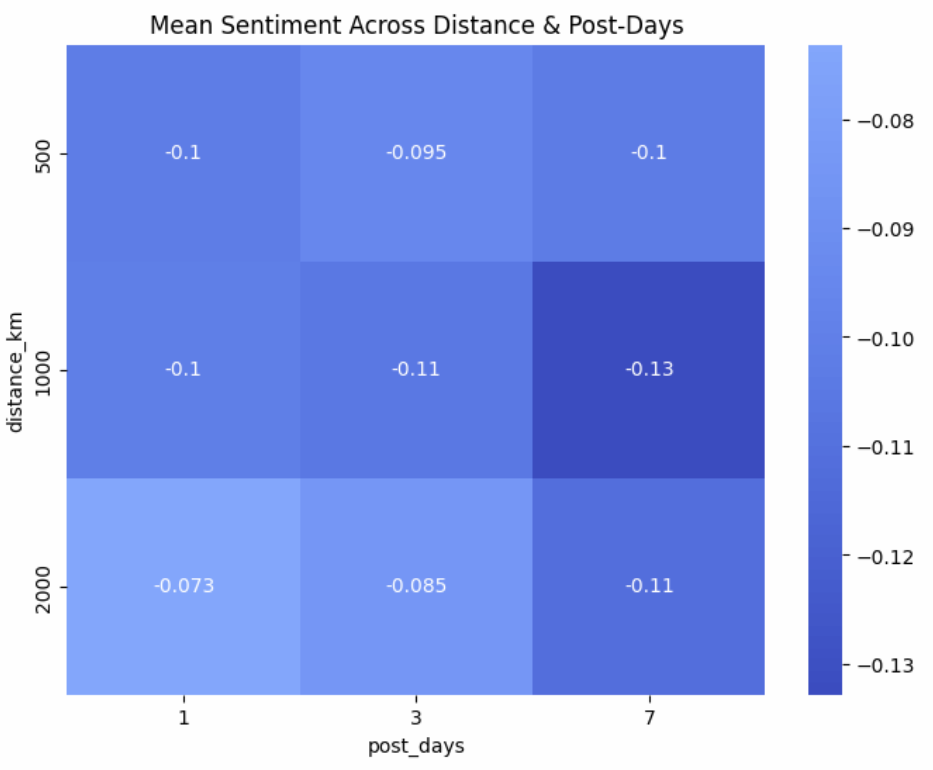
\includegraphics[width=10cm]{images/climatechangepulse7.PNG}
\caption{Correlation matrix of the mean sentiment across distance (km) and days post-disaster}
\end{figure}



The analysis reveals several key insights about the relationship between disasters and public sentiment on Twitter. First, sentiment becomes more negative as the distance threshold increases, suggesting that tweets closer to disaster locations reflect stronger emotional responses. This aligns with the expectation that proximity to a disaster intensifies public concern and emotional expression.



Second, the time window significantly influences sentiment. Pre-event sentiment becomes more negative as the number of days before a disaster increases, potentially reflecting growing anxiety or anticipation. Post-event sentiment also trends more negatively over time, possibly due to prolonged discussions or the accumulation of negative news.

A surprising finding is the stark contrast in sentiment between different stances. Deniers exhibit the most negative sentiment, which may reflect frustration or skepticism toward climate change discourse. Believers, while also negative, show less extreme sentiment, possibly indicating a more measured or concerned tone. Neutral users, as expected, exhibit the least negative sentiment, suggesting a lack of strong emotional investment.

\begin{figure}[H]
\centering
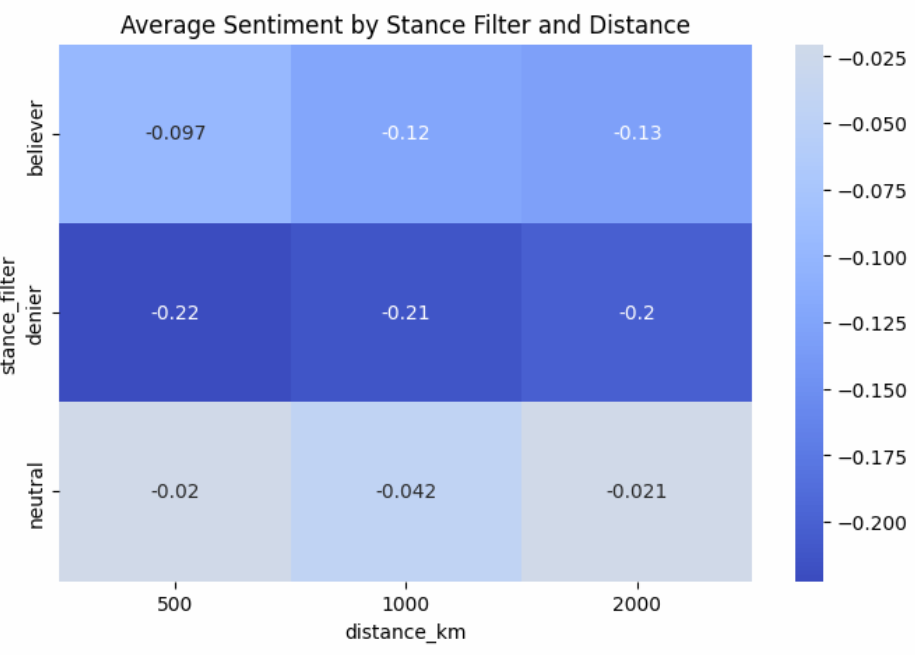
\includegraphics[width=10cm]{images/climatechangepulse9.PNG}
\caption{Correlation matrix of the average sentiment by stance and distance}
\end{figure}

The biggest effect on results appears to be the combination of distance and stance. Tweets closer to disasters from deniers show the most negative sentiment, while neutral users remain relatively unaffected. This suggests that emotional responses to disasters are not only influenced by proximity but also by individuals' pre-existing beliefs about climate change.

\begin{figure}[H]
\centering
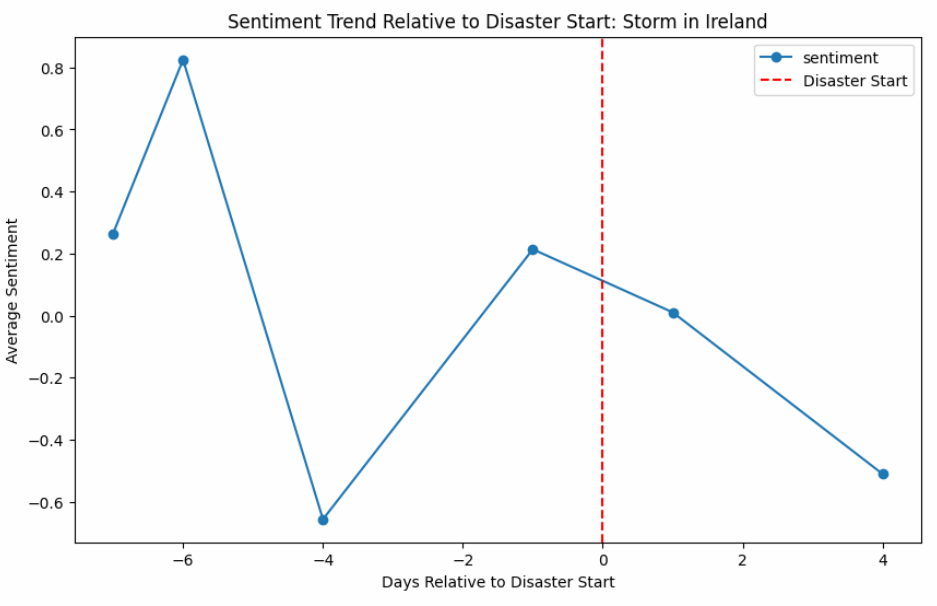
\includegraphics[width=10cm]{images/climatechangepulse8.PNG}
\caption{Line plot of sentiment across time. The example shows the changes in tweet sentiment across days before and after the disaster.}
\end{figure}

Overall, the experiment highlights the importance of carefully selecting distance and time parameters to capture meaningful sentiment patterns. It also underscores the role of stance in shaping public discourse around disasters, offering valuable insights for targeted communication strategies.

\section{Methodology Comparison}\label{sec5}
\subsection{Methodology A}\label{subsec11}
A similar project was “A novel sentiment analysis framework for monitoring the evolving public opinion in real-time: Case study on climate change.” by Barachi, May El, et. al. The authors had access to data similar to the climate change twitter dataset and some api for data collection(which we didn’t readily have). It employs a Bi-directional LSTM that assigns and categorizes sentiments into different categories. Today state-of-the-art models would improve the quality of the performance. Their task was training a model specifically to assign labels, which we build off of.

We used already labeled data from a similar model in order to drive analysis and understanding of the data, and draw conclusions from it. We have different scopes, as they were trying to collect data while we focused on data analysis. They reported the accuracy for different emotions and positions. Our application has the potential for internet-users and experts alike to offer critique on the issue.

\subsection{Methodology B}\label{subsec12}
Lu, Yafeng, et. al. addresses a similar problem of using social media data to see how disasters impact sentiment. Using the Ebola Twitter dataset, they are primarily concerned about investigating sentiment trends and behaviors in geo-located twitter data. Their approach follows by using pre-trained classifiers to label the raw data with a sentiment score, assigning labels based on a majority vote, and then taking the twitter data classes and passing into the entropy function. They aim to primarily investigate the quantifiable levels of disagreement among the classes.

Our project is building off this, because we have a UI and more factors in our analysis. Since we have a UI it is more accessible. Also, we were concerned about investigating the behaviors of deniers and believers.

\subsection{Methodology C}\label{subsec13}
A relevant study which aims to address the analysis of climate change discourse on social media examines sentiments expressed in Twitter interactions related to climate change, analyzing 92,474 tweets to assess sentiment polarity and underlying topics (Mouronte-Lopez and Subiran, 2022). The study employs algorithms such as VADER and TextBlob, alongside unsupervised machine learning techniques, to determine sentiment polarity and utilizes Latent Dirichlet Allocation (LDA) for topic modeling. The findings reveal that discussions on climate change are predominantly negative across various topics, including activism, biodiversity, and sustainability. Not only this, but they also explore differences in sentiment by geography, gender, and account type. Our project builds upon this foundation by providing an interactive web tool that visualizes natural disasters on a world map, overlaid with relevant tweets. Users can explore disasters by year and location, with red dots indicating recorded events.

\subsection{Methodology D}\label{subsec14}
The survey by Singh, et al., "Agentic Retrieval-Augmented Generation: A Survey on Agentic RAG," offers a comprehensive overview of various RAG system implementations and their respective strengths and weaknesses. The key goal of their paper is to discuss the advantages of designing one framework over another, which resonates directly with our development journey.

Our solution has undergone several iterations of RAG-based systems, notably exploring the naive RAG approach, to then pivoting towards an agentic framework. Given the static and tabular nature of our external data, we discovered that traditional document chunking and storage weren't the most effective solution. Instead, we investigated using RAG techniques to generate SQL queries to assist in filtering our data at a large scale. The inherent iterative nature and multi-domain task strengths of agentic systems show promising results for building a conversational chatbot in our use case, and thus, we've opted to integrate this system into our web application.

\section{Conclusions}\label{section6}
\subsection{Limitations and Improvements}\label{subsec15}
One limitation of our project is the reliance on pre-labeled data from the Climate Change Twitter Dataset, which may contain inherent biases from the original labeling process. Additionally, many tweets lack geospatial information, limiting the scope of our disaster-to-sentiment correlation analysis. The embedded tweet feature, while useful, restricts access to older or deleted tweets, potentially omitting valuable data. Furthermore, our current sentiment analysis does not fully capture nuanced emotions or the context behind tweets, which could affect the depth of our insights.

If given more time, we would improve the project by incorporating more robust natural language processing techniques, such as fine-tuned transformer models, to enhance sentiment classification. We’d also explore geolocation inference methods to fill in missing location data. Expanding the dataset to include real-time data collection via APIs would provide more dynamic insights. Finally, adding advanced data visualization tools would improve user interaction and data interpretation.

\subsection{Concluding Remarks}\label{subsec16}
Climate Change Pulse bridges the gap between climate change discourse and real-world disaster impacts through data visualization and sentiment analysis. By mapping tweets alongside natural disasters, we provide unique insights into public perception. Our tool fosters awareness and can inform policy discussions, highlighting how climate events influence global sentiment.


\newpage


\section{References}\label{sec9} Torres, Bustos Emmanuel. (n.d.). Global temperature D3.js data visualization. GitHub. https://github.com/ema2159/global-temperature.

Thunberg, G. (2023). The Climate Book. New York, Penguin Press.

Barachi, May El, et. al. “A novel sentiment analysis framework for monitoring the evolving public opinion in real-time: Case study on climate change.” ScienceDirect, https://www.sciencedirect.com/science/article/abs/pii/S0959652621020382. 

Lu, Yafeng, et. al. “Visualizing Social Media Sentiment in Disaster Scenarios.” ACM, https://dl.acm.org/doi/abs/10.1145/2740908.2741720.

Mouronte-López, M., \& Subirán, M. (2022). What do Twitter users think about climate change? Characterization of Twitter interactions considering geographical, gender, and account typologies perspectives. Weather, Climate, and Society, 14(4), 865–877. https://doi.org/10.1175/WCAS-D-21-0163.1

Lu, Yafeng, Hu, Xia, et. al. “Visualizing Social Media Sentiment in Disaster Scenarios.”https://archives.iw3c2.org/www2015/documents/proceedings/companion/p1211.pdf

Aditi Singh, Abul Ehtesham, et. al. “AGENTIC RETRIEVAL-AUGMENTED GENERATION: A SURVEY ON AGENTIC RAG” https://arxiv.org/html/2501.09136v1

Anderson, M., Faverio, M., \& Gottfried, J. (2023, December 11). Teens, social media 
and technology 2023. Pew Research Center: Internet, Science \& Tech. https://www.pewresearch.org/internet/2023/12/11/teens-social-media-and-technology-2023/
% \section{3}\label{sec3}
% \subsection{3.1}\label{subsec2}
% ...

%%===========================================================================================%%
%% If you are submitting to one of the Nature Portfolio journals, using the eJP submission   %%
%% system, please include the references within the manuscript file itself. You may do this  %%
%% by copying the reference list from your .bbl file, paste it into the main manuscript .tex %%
%% file, and delete the associated \verb+\bibliography+ commands.                            %%
%%===========================================================================================%%

%%\bibliography{sn-bibliography}% common bib file
%% if required, the content of .bbl file can be included here once bbl is generated
%%\input sn-article.bbl

\end{document}
